\chapter{绪论}
\label{chp1}

\section{雷达的基本概念}
雷达是英文 Radio Detection and Ranging(Radar)的缩写的英译,即用无线电波的反射信号发现目标并测定其空间位置、移动方向、速度、相对距离以及大概形状的电子设备。作为一种重要的探测手段,雷达被广泛应用于航空与航海导航、军事侦察和预警、气象观测以及太空探索等领域。

严格来说,雷达的研发工作始于20世纪30年代,最初是为了探测敌方飞机和舰船而设计的,但雷达的基本概念却可以追溯到半个多世纪前。在1864年,麦克斯韦(James Clerk Maxwell)提出了电磁波的理论,给出了著名的麦克斯韦方程组,从理论上证明了光是一种特殊的电磁波。该理论的一个延伸是,电磁波也可以像电磁波一样被金属物体反射、被电介质折射。随后赫兹(Heinrich Hertz)在1887年使用波长为66厘米(对应于大约 455MHz)的无线电波成功地实验验证了这一结论,并于1888年发表了相关论文。

实验装置如\cref{fig_chp1_hertz}所示,主要由一个发射天线和一个接收天线组成。其中发射天线是由两个黄铜球连接的金属棒构成,中间留有一个小间隙。当接通电源时,电流在金属棒之间产生振荡,从而在空间中产生无线电波。这些无线电波会在空间中传播,并被金属板反射回来,形成驻波。接收天线则是一个有开口的金属环,它可以接收到反射回来的无线电波,并在开口处产生火花。通过移动接收天线的位置,可以观察到火花的强度变化,从而得到无线电波的波长,结合频率可以计算出电磁波的传播速度,进而验证麦克斯韦方程组的正确性。

\begin{figure}[htb!]
    \centering
    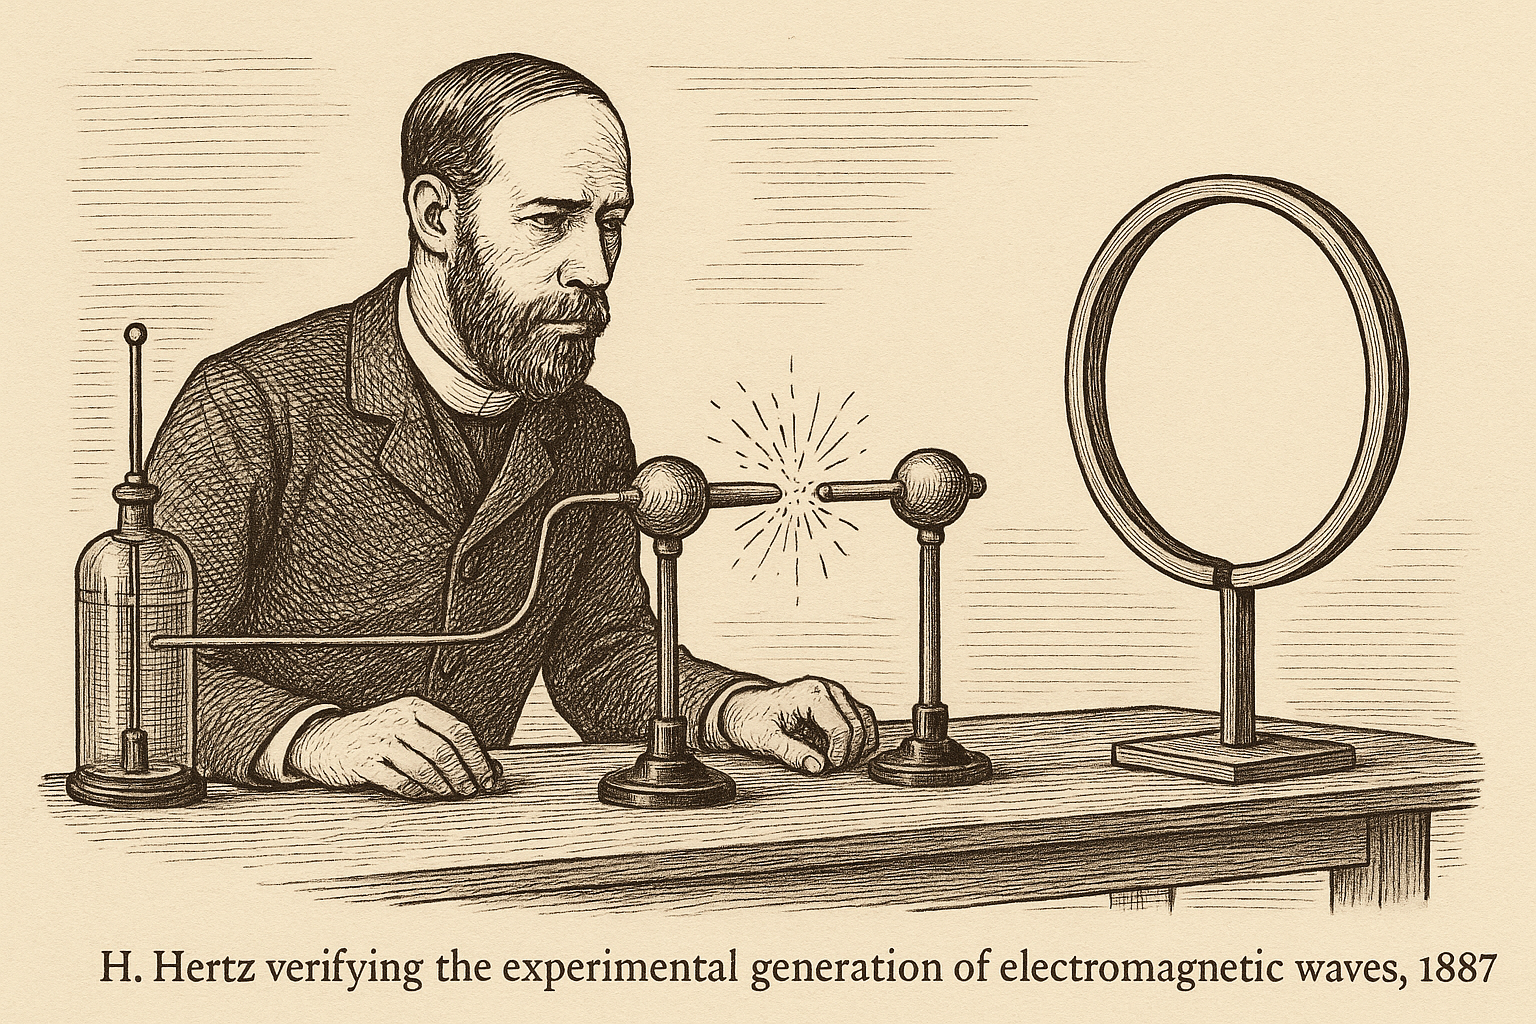
\includegraphics[width=.6\textwidth]{./img/chp1/hertz_experiment.png}
    \caption{赫兹的实验装置示意图}
    \label{fig_chp1_hertz}
\end{figure}

雷达利用的便是电磁波的反射特性,通过发射电磁波并接收其反射信号来探测目标物体的位置、方位和速度等信息。雷达系统通常包括发射机、接收机、天线和信号处理单元等部分。发射机产生高频电磁波信号,通过天线向外发射。当电磁波遇到目标物体时,会发生反射,反射信号被天线接收并传输到接收机进行处理。通过分析反射信号的时间延迟和频率变化等特征,可以计算出目标物体的距离、速度和方向等信息。

\section{雷达工作原理}

\subsection{基本组成}
雷达系统的主要组成部分包括发射机、接收机、天线、波形产生器和信号处理单元等,如\cref{fig_chp1_radar_system}所示。

\begin{figure}[htb!]
    \centering
    % \includegraphics[width=.4\textwidth]{./img}
    \begin{tikzpicture}
        \tikzset{
            myblock/.style={
                    rectangle, draw, minimum width=2cm, minimum height=1cm, rounded corners, thick
                }
        }

        \node (transmitter) [myblock, fill=c1!60, draw=c1] at (0, 0) {发射机};
        \node (receiver) [myblock, fill=c2!60] at (0, -3) {接收机};
        \node (antenna) [myblock, fill=c3!60] at (-3, -1.5) {天线};
        \node (waveform_generator) [myblock, fill=c4!60] at (3, 0) {波形产生器};
        \node (signal_processing) [myblock, fill=c5!60] at (3, -3) {信号处理单元};

        \draw[-latex, thick] (transmitter) -- (antenna);
        \draw[-latex, thick] (antenna) -- (receiver);
        \draw[-latex, thick] (receiver) -- (signal_processing);
        \draw[-latex, thick] (waveform_generator) -- (transmitter);
    \end{tikzpicture}
    \caption{雷达系统的基本组成}
    \label{fig_chp1_radar_system}
\end{figure}

整个雷达系统的工作流程如下:
\begin{enumerate}
    \item \textbf{波形产生}:波形产生器生成特定的电磁波信号,通常是脉冲信号或连续波信号。
    \item \textbf{发射}:发射机将生成的电磁波信号放大,并通过天线向外发射。
    \item \textbf{接收}:当电磁波遇到目标物体时,会发生反射,反射信号被天线接收并传输到接收机,接收机将接收到的信号进行放大和滤波,以提高信噪比。
    \item \textbf{信号处理}:信号处理单元对接收到的信号进行分析和处理,以提取目标信息,如距离、速度和方位等。
    \item \textbf{显示与控制}:处理后的目标信息可以通过显示器或其他输出设备进行显示,同时可以根据需要进行控制和调整。
\end{enumerate}

\subsection{工作频率}

雷达的工作频率范围非常广泛,从几千赫兹(kHz)到几百吉赫兹(GHz)不等。工程上将雷达的工作频率划分为多个频率,\cref{tab_chp1_radar_frequency}给出了常见的雷达工作频率范围、对应的波段名称以及主要应用场景和特点。

\begin{table}[htb!]
    \centering
    \caption{常见雷达工作频率范围及应用}
    \label{tab_chp1_radar_frequency}
    \small
    \begin{tabular}{c|c|p{7cm}}
        \hline
        波段名称 & 频率范围           & 主要应用场景和特点                                                                                                      \\
        \hline
        \hline
        HF   & 3 - 30 MHz     & 短波具有在地面与电离层之间多次反射的特性(天波),适用于超视距、超远程雷达工作;但电波传播稳定性差,电磁频谱拥挤,易受干扰,不易辨别真伪目标,一般雷达不采用
        \\
        \hline
        VHF  & 30 - 300 MHz   & 米波雷达具有大天线口径、高辐射功率、传播衰减小和不受气象条件影响和建造费用相对较低的优点。米波是监视卫星、洲际导弹的大型超远程雷达的重要波段。它也可用于一般简单的中、近程监视雷达。但频段频谱拥挤与通信频段猫短,一般较少用 \\ \hline
        UHF  & 300 - 1000 MHz & 适用于远程监视雷达,但因电视频段占用而很少采用                                                                                        \\
        \hline
        L    & 1 - 2 GHz      & 此频段的天线发射增益、天线口径、发射功率、接收机噪声性能、抗干扰性能等都较适中,是中、远程对空监视雷达常用的重要波段                                                     \\
        \hline
        S    & 2 - 4 GHz      & 为对空搜索监视雷达和导航雷达的常用波段,尤其是对空监视跟踪用的中程雷达标                                                                           \\
        \hline
        C    & 4 - 8 GHz      & 为精密监视雷达、精密跟踪雷达和中远程控制雷达常用的重要波段;但因气象干扰较明显,常为气象雷达所采用                                                              \\
        \hline
        X    & 8 - 12 GHz     & 为中、近程武器控制、跟踪、对海搜索、导航、机载搜索攻击、战略侦察、交通管制等近程雷达常用的重要波段。气象干扰明显,还常为气象雷达采用                                             \\
        \hline
        Ku   & 12 - 18 GHz    & \multirow{1}{7cm}{该波段的雷达有良好的分辨力、互相干扰小;但功率小、易受噪声影响、传播衰减和气象条件影响较大,仅适用于近程搜索、监视、武器跟踪和制导}                           \\
        \cline{1-2}
        K    & 18 - 27 GHz    &                                                                                                                \\
        \cline{1-2}
        Ka   & 27 - 40 GHz    &                                                                                                                \\
        \hline
        V    & 40 - 75 GHz    & \multirow{3}{7cm}{毫米波雷达功率低,噪声大,大气吸收和气象干扰严重,作用距离近,但分辨率较高,在自动驾驶中使用较多}                                            \\
        \cline{1-2}
        W    & 75 - 110 GHz   &                                                                                                                \\
        \cline{1-2}
        mm   & 110 - 300 GHz  &                                                                                                                \\
        \hline
    \end{tabular}
\end{table}

\subsection{目标探测}


\section{电磁波传播特性}

电磁波在自由空间中以光速 $c$ 传播,具有许多典型特性,如直线传播、反射、折射、衍射、散射和吸收等。这些特性直接决定了雷达信号的传播路径与能量分布。

\subsection{电磁波的反射}

当电磁波遇到不同介质界面时,会发生部分反射。对于平滑金属目标(如飞机、舰船、汽车等),主要产生镜面反射(如\cref{fig_chp1_reflection_1}所示),这是雷达探测的主要基础。而对于粗糙或尺寸与波长相当的目标(如云层、雨滴、雪花、林地等),会出现明显的漫反射现象(如\cref{fig_chp1_reflection_2}所示)。

\begin{figure}[htb!]
    \centering
    \begin{subfigure}{.4\textwidth}
        \centering
        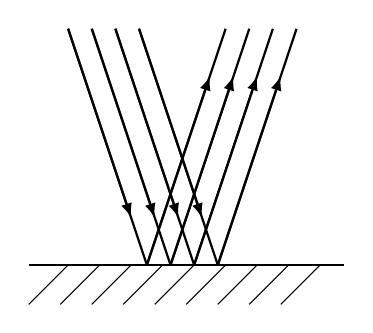
\begin{tikzpicture}
            \draw[thick] (-3, 0) -- (1, 0); % Ground line
            \foreach \i in {-3, -2.6, ..., 0.5} {
                    \draw[] (\i, -0.5) -- (\i+0.5, 0); % Vertical lines
                }
            \foreach \i in {-2.5, -2.2, -1.9, -1.6} {
                    \draw[thick, -latex] (\i, 3) -- (\i +0.8, 0.6);
                    \draw[thick] (\i, 3) -- (\i+1, 0);
                }
            \foreach \i in {-2.5, -2.2, -1.9, -1.6} {
                    \draw[thick, -latex] (\i+1, 0) -- (\i+1.8, 2.4);
                    \draw[thick] (\i+1, 0) -- (\i+2, 3);
                }
        \end{tikzpicture}
        \caption{}
        \label{fig_chp1_reflection_1}
    \end{subfigure}
    \begin{subfigure}{.4\textwidth}
        \centering
        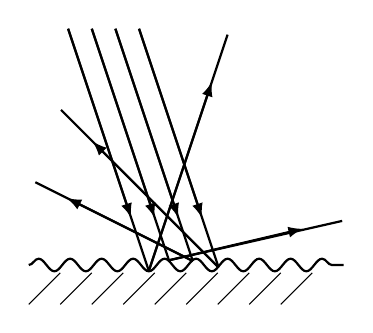
\begin{tikzpicture}
            \draw[thick,decorate,decoration={snake,amplitude=0.8mm,segment length=4mm}] (-3, 0) -- (1, 0); % Ground line
            \foreach \i in {-3, -2.6, ..., 0.5} {
                    \draw[] (\i, -0.5) -- (\i+0.4, -0.1); % Vertical lines
                }

            \foreach \i in {-2.5, -2.2, -1.9, -1.6} {
                    \draw[thick, -latex] (\i, 3) -- (\i +0.8, 0.6);
                }
            \draw[thick] (-2.5, 3) -- (-2.5+1+0.025, 0-0.075);
            \draw[thick, -latex] (-2.5+1+0.025, 0-0.075) -- (-2.5+1+0.025+0.8, 0-0.075+2.4);
            \draw[thick] (-2.5+1+0.025, 0-0.075) -- (-2.5+1+0.025+1, 0-0.075+3);

            \draw[thick] (-2.2, 3) -- (-2.2+1-0.02, 0+0.06);
            \draw[thick] (-2.2+1-0.02, 0+0.06) -- (-2.5+1-0.02+2.5, 0+0.06+0.5);
            \draw[thick, -latex] (-2.2+1-0.02, 0+0.06) -- (-2.5+1-0.02+2, 0+0.06+0.4);

            \draw[thick] (-1.9, 3) -- (-1.9+1-0.017, 0+0.051);
            \draw[thick] (-1.9+1-0.017, 0+0.051) -- (-1.9+1-0.017-2, 0+0.051+1);
            \draw[thick, -latex] (-1.9+1-0.017, 0+0.051) -- (-1.9+1-0.017-1.6, 0+0.051+0.8);

            \draw[thick] (-1.6, 3) -- (-1.6+1+0.01, 0-0.03);
            \draw[thick] (-1.6+1+0.01, 0-0.03) -- (-1.6+1+0.01-2, 0-0.03+2);
            \draw[thick, -latex] (-1.6+1+0.01, 0-0.03) -- (-1.6+1+0.01-1.6, 0-0.03+1.6);
        \end{tikzpicture}
        \caption{}
        \label{fig_chp1_reflection_2}
    \end{subfigure}
    \caption{电磁波的反射示意图 (a) 镜面反射 (b) 漫反射}
    \label{fig_chp1_reflection}
\end{figure}

不同的雷达系统会根据目标的反射特性选择合适的工作频率和波形。例如,气象雷达通常使用较低频率,以便更好地探测云层和降水;而军事雷达则可能使用更高频率,以提高分辨率和探测精度。

此外,隐身飞机为了降低被雷达探测的概率,通常会采用特殊的设计和材料来减少雷达波的反射。根据电磁波的反射特性,目前主流的隐身技术主要包括以下两种:
\begin{enumerate}
    \item \textbf{外形优化设计}:通过机身外形的精细设计,采用倾斜表面和尖锐棱角结构,尽可能避免出现直角和垂直面,以显著降低雷达波的直接反射。
    \item \textbf{结构与涂层设计}:飞机内部采用蜂窝状或多孔结构,以增强对雷达波的吸收;同时在机体表面涂覆特殊材料(如吸波材料或漫反射涂层),进一步降低雷达波的反射强度。
\end{enumerate}

利用镜面反射,还可以设计一种特殊的器械,叫作角反射器又名雷达反射器,简称角反。角反可以以将入射的电磁波反射回原方向,通常由三个互相垂直的平面组成,如\cref{fig_chp1_corner_reflector}所示。

\begin{figure}[htb!]
    \centering
    \begin{subfigure}{.3\textwidth}
        \centering
        \includegraphics[width=.8\textwidth]{./img/chp1/corner_reflector_1.tikz}
        \caption{}
        \label{fig_chp1_corner_reflector_1}
    \end{subfigure}
    \begin{subfigure}{.3\textwidth}
        \centering
        \includegraphics[width=.9\textwidth]{./img/chp1/corner_reflector_2.tikz}
        \caption{}
        \label{fig_chp1_corner_reflector_2}
    \end{subfigure}
    \caption{角反射器示意图 (a) 结构示意 (b) 工作原理}
    \label{fig_chp1_corner_reflector}
\end{figure}

事实上,角反在生活中非常常见。比如自行车的尾灯上通常会有一个小的角反射器(如\cref{fig_chp1_bike}所示),用于提高夜间行车的安全性。仔细观察可以发现,这种角反是由大量的小型角反组成的。

\begin{figure}[htb!]
    \centering
    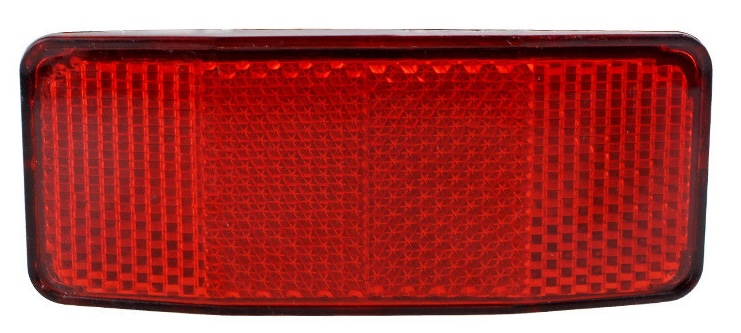
\includegraphics[width=.4\textwidth]{./img/chp1/bike.jpeg}
    \caption{自行车尾部的角反射器}
    \label{fig_chp1_bike}
\end{figure}

由于角反可以有效地将入射的电磁波反射回原方向,因此可以提供稳定、明确的强回波信号,通常被用作雷达系统的校准目标,检验雷达设备的测距精度、方向精度和灵敏度。在航海与航空领域,角反射器常用于标识特定位置,如航道、海岸线或机场跑道周围,为雷达导航提供明确的位置标识,提高导航的准确性与安全性。


\subsection{电磁波的折射}

电磁波在不同介质中传播时,会发生折射现象。折射是指电磁波在穿过介质界面时,传播方向发生改变的现象。折射的程度取决于入射角和介质的折射率。折射率是描述介质对电磁波传播影响的一个重要参数,定义为电磁波在真空中的传播速度与光在该介质中的传播速度之比,即
\begin{equation}
    n = \frac{c}{v}.
    \label{eq:refraction_index}
\end{equation}

折射是一种常见现象,可以用斯涅尔定律(Snell's Law)来描述。斯涅尔定律表明,当电磁波从一种介质进入另一种介质时,入射角 $\theta_1$、折射角 $\theta_2$ 和两种介质的折射率 $n_1$、$n_2$ 之间满足以下关系:
\begin{equation}
    n_1 \sin \theta_1 = n_2 \sin \theta_2.
    \label{eq:snell_law}
\end{equation}

当电磁波以一个较大的入射角,从折射率较大的介质进入折射率较小的介质时,可能会出现
\[
    n_1 \sin \theta_1 > n_2,
\]
的情况。此时,即便是\( \theta_2 \) 达到 90°,也无法满足\cref{eq:snell_law},从而导致电磁波无法进入到低折射率介质中,而是全部反射回来。这种现象被称为全反射(Total Internal Reflection)。全反射的条件是入射角大于临界角 $\theta_c$,临界角可以通过以下公式计算:
\begin{equation}
    \sin \theta_c = \frac{n_2}{n_1}.
    \label{eq:critical_angle}
\end{equation}

光纤通信就是利用全反射原理实现的。光纤的核心部分具有较高的折射率,而包裹在外面的包层则具有较低的折射率。当光线以适当的入射角进入光纤时,会发生全反射,从而使光信号在光纤中传播而不损失能量。

在雷达系统中,折射现象也会影响电磁波的传播路径。在海面附近,由于水汽蒸发,会导致近海面小范围内大气湿度随高度锐减,从而形成一个较强的折射率梯度。或是在地面附近,出现逆温层,此时在一个较小的高度范围内,温度随高度增加而迅速升高,同样也会形成一个较强的折射率梯度。

\begin{figure}[htb!]
    \centering
    \includegraphics[width=.7\textwidth]{./img/chp1/atmosphere_duct.tikz}
    \caption{大气波导示意图}
    \label{fig_chp1_atmosphere_duct}
\end{figure}

如\cref{fig_chp1_atmosphere_duct}所示,此时,电磁波在传播时,由于折射率梯度的存在,传播曲线会发生弯曲,导向海面或地面,并被反射。反射后,电磁波的路径会再次发生弯曲,入射角逐渐增大,直到出现全反射现象,将电磁波再次反射回地面。重复这一过程,电磁波便可以在大气层中沿着地面或海面传播很远的距离,而不会明显衰减。这种现象被称为大气波导(Atmospheric Ducting),也称为大气波导效应。除此以外,大气波导也可能发生在海拔数十米或数百米的空中,基本原理与上述类似,不再赘述。需要注意的是,\cref{fig_chp1_atmosphere_duct}仅为示意图,其中大气的折射率变化并不连续,仅为简化说明而作的分段近似。

当出现大气波导现象时,雷达可以探测到地平线以下的目标。尽管能够探测到目标,但却很难精确地测量目标的距离。如\cref{fig_chp1_radar_ducting}所示,由于大气波导效应,电磁波会沿着地表或海面传播,形成一个弯曲的路径,从而能够探测到地平线以下的目标。
\begin{figure}[htb!]
    \centering
    \includegraphics[width=.6\textwidth]{./img/chp1/radar_atmosphere.tikz}
    \caption{雷达超视距探测示意图}
    \label{fig_chp1_radar_ducting}
\end{figure}

\subsection{自由空间路径损耗与大气衰减}

自由空间衰减(Free-Space Path Loss)则是指电磁波在自由空间中传播时,由于距离的增加而导致的功率损耗,通常被定义为发射功率与接收功率之间的比率。设有一个发射功率为 $P_t$ 的天线,以球面波形式向外辐射电磁波,则在距离 $d$ 处该电磁波的功率密度 $S$ 可以表示为:
\begin{equation}
    S = \frac{P_t}{4 \pi d^2}.
    \label{eq:free_space_power_density}
\end{equation}
而在此处的接收天线接收到的功率 $P_r$ 则与天线的有效面积 $A_e$ 有关,通常可以表示为:
\begin{equation}
    P_r = S A_e = \frac{P_t A_e}{4 \pi d^2}.
    \label{eq:free_space_received_power}
\end{equation}
其中,$A_e$ 是接收天线的有效面积,对于一个各向增益都为1的理想天线,其有效面积可以表示为:
\begin{equation}
    A_e = \frac{\lambda^2}{4 \pi},
    \label{eq:effective_area}
\end{equation}
其中 $\lambda$ 是电磁波的波长。
将\cref{eq:effective_area}代入\cref{eq:free_space_received_power},可以得到接收功率与发射功率之间的关系:
\begin{equation}
    L = \frac{P_t}{P_r} = \left( \frac{4 \pi d}{\lambda} \right)^2 = \left( \frac{4 \pi f d}{c} \right)^2.
    \label{eq:free_space_received_power_final}
\end{equation}
其中,$L$ 即为自由空间路径损耗。

从\cref{eq:free_space_received_power_final}可以看出,自由空间路径损耗与频率 $f$ 的平方成正比。所以想要进行远距离的探测,通常需要使用低频段的电磁波。但低频段的电磁波分辨率较低,无法提供足够的细节信息。因此,在自动驾驶、无人机等应用中,通常会使用高频的毫米波雷达(如24GHz或77GHz),以获得更高的分辨率和精度。

除此以外,电磁波在大气中传播时还会受到大气衰减的影响。大气衰减是指电磁波在大气中传播时,由于大气中的水汽、氧气、二氧化碳等分子对电磁波的吸收和散射作用,导致信号强度的衰减。需要注意的是,大气衰减是指相对于自由空间路径损耗的大气导致的额外功率损耗。大气衰减与频率有关,通常在高频段(如微波和毫米波)更为显著。如\cref{fig_chp1_gaspl}所示,随着频率的增加,大气衰减会显著增加,并且湿空气的衰减比干燥空气更为明显。

\begin{figure}[htb!]
    \centering
    \includegraphics[width=.5\textwidth]{./img/chp1/gaspl.tikz}
    \caption{大气衰减曲线(距离1千米,温度$15^\circ$C,气压 $1013$ hPa)}
    \label{fig_chp1_gaspl}
\end{figure}

严格来说,大气本身只能对电磁波产生吸收或散射作用,能量并不会凭空增加。然而,从\cref{fig_chp1_gaspl}可以观察到,衰减数值在某些情况下可能为负值。也就是说,相对于在自由空间中传播,此时电磁波在大气中传播反而损耗更小。这主要是因为,在大气(尤其是近地层)中,温度、湿度等因素引起的折射率梯度会导致电磁波沿地表被导引传播,类似于波导效应,使得能量分布更加集中。因此,即便在较远的距离处,也能够接收到较强的信号。

\subsection{色散现象与多径效应}
电磁波在大气中传播除了会产生传输损耗(衰减)之外,还可能会产生失真。一般来说,产生失真的原因有两个,介质的色散现象和随机多径传输导致的干涉效应。

对于同一个介质,不同频率的电磁波在该介质中的传播速度有可能是不同的。这就会导致在传播的过程中,雷达发射的信号波形产生畸变,这种现象称为色散现象(Dispersion)。色散现象的一个典型例子是光在玻璃中的传播。当白光通过棱镜时,不同波长的光会以不同的速度传播,从而导致光线分散成彩虹色谱。如果我们将传播介质看作是一个线性系统,那么该系统的频率响应是非线性相位的。而对于一个非线性相位的系统,其输出信号的波形相较于输入信号波形会发生畸变。

不过好在大气对常见的雷达工作频率的色散效应并不明显,通常可以忽略不计。比如最靠近地表的对流层,其对20GHz以下的电磁波基本上是无色散的。

此外,多径效应(Multipath Effect),则是指电磁波在传播过程中,由于遇到障碍物或地形的反射、折射和散射等作用,导致同一信号在不同路径上到达接收天线的现象,如\cref{fig_chp1_multipath}所示。多径效应会导致接收信号的相位和幅度发生变化,从而引起信号的干扰和失真。严重时,不同路径上的信号可能会相互抵消,导致接收信号的强度显著降低。

\begin{figure}[htb!]
    \centering
    \includegraphics[width=.5\textwidth]{./img/chp1/multipath.tikz}
    \caption{多径效应示意图}
    \label{fig_chp1_multipath}
\end{figure}
